\documentclass{article}
\usepackage{amsmath}
\usepackage{amsfonts}
\usepackage{geometry}
\usepackage{xcolor}
\usepackage{tikz}
\usepackage{pgfplots} % For creating graphs
\pgfplotsset{compat=1.18}
\usetikzlibrary{shapes.geometric, arrows, positioning}
\usepackage{listings} % For code syntax highlighting
\usepackage{xcolor} % Already included but ensure for listings

% Configure TypeScript syntax highlighting
\lstdefinelanguage{TypeScript}{
  keywords={const, let, var, function, return, if, else, for, while, break, continue, true, false, null, undefined, number, string, boolean, any, void, interface, type, class, extends, implements, public, private, protected, static, readonly, abstract, async, await, import, export, from, as, default},
  keywordstyle=\color{blue}\bfseries,
  ndkeywords={console, log},
  ndkeywordstyle=\color{purple}\bfseries,
  identifierstyle=\color{black},
  sensitive=true,
  comment=[l]{//},
  morecomment=[s]{/*}{*/},
  commentstyle=\color{gray}\ttfamily,
  stringstyle=\color{red}\ttfamily,
  morestring=[b]',
  morestring=[b]",
  morestring=[b]`,
}

\lstset{
  language=TypeScript,
  basicstyle=\ttfamily\footnotesize,
  numbers=left,
  numberstyle=\tiny\color{gray},
  stepnumber=1,
  numbersep=5pt,
  backgroundcolor=\color{gray!5},
  showspaces=false,
  showstringspaces=false,
  showtabs=false,
  frame=single,
  rulecolor=\color{black},
  tabsize=2,
  captionpos=b,
  breaklines=true,
  breakatwhitespace=false,
  escapeinside={\%*}{*\%},
  aboveskip=\bigskipamount,
  belowskip=\bigskipamount
}
\geometry{margin=1in}

% Define a command for code variables
\newcommand{\code}[1]{\textcolor{blue}{\texttt{#1}}}

\title{Energy Calculations for PTAC vs PTHP Systems}
\author{EDK Energy Insight Platform}
\date{\today}

\begin{document}

\maketitle

\section{Introduction}

This document outlines the energy calculations for comparing Packaged Terminal Air Conditioner (PTAC) and Packaged Terminal Heat Pump (PTHP) systems, using the standardized variable names from our codebase.

\section{PTAC System Calculations}

\subsection{Per-Unit Constants}

The system uses fundamental constants for PTAC units in original units and their MMBtu equivalents:

\begin{itemize}
    \item \code{annualUnitThermsHeatingPTAC}: 255 therms per year per unit for heating
    \item \code{annualUnitKwhCoolingPTAC}: 16,000 kWh per year per unit for cooling
    \item \code{annualUnitMMBtuHeatingPTAC}: 25.5 MMBtu per year per unit for heating
        \begin{itemize}
            \item Converted from 255 therms × 0.1 MMBtu/therm = 25.5 MMBtu
        \end{itemize}
    \item \code{annualUnitMMBtuCoolingPTAC}: 5.459427 MMBtu per year per unit for cooling
        \begin{itemize}
            \item Converted from 16,000 kWh × 0.003412 MMBtu/kWh = 5.459427 MMBtu
        \end{itemize}
\end{itemize}

\subsection{Building-Level Calculations}

For a building with multiple units, we calculate both MMBtu and original unit values:

\subsubsection{MMBtu Building Totals}
\begin{equation}
\code{annualBuildingMMBtuCoolingPTAC} = N_{ptacUnits} \times \code{annualUnitMMBtuCoolingPTAC}
\end{equation}

\begin{equation}
\code{annualBuildingMMBtuHeatingPTAC} = N_{ptacUnits} \times \code{annualUnitMMBtuHeatingPTAC}
\end{equation}

\begin{equation}
\code{annualBuildingMMBtuTotalPTAC} = \code{annualBuildingMMBtuCoolingPTAC} + \code{annualBuildingMMBtuHeatingPTAC}
\end{equation}


\section{PTHP System Calculations}

\subsection{Heating Energy Conversion with Building-Specific EFLH}

For PTHP systems, the heating energy is calculated using building-specific Equivalent Full Load Hours (EFLH) derived from PLUTO data, combined with PTHP heating capacity and coefficient of performance:

\subsubsection{Step 1: Calculate Annual Building kWh for PTHP Heating}

The annual building heating consumption in kWh is calculated using the detailed equation:

\begin{equation}
\code{annualBuildingkWhHeatingPTHP} = \frac{\code{heatingCapacityPTHP}}{3.412} \times \frac{1}{\code{pthpCOP}} \times \text{EFLH} \times N_{ptacUnits}
\end{equation}

Where:
\begin{itemize}
    \item \code{heatingCapacityPTHP}: 8 KBtu (constant heating capacity per PTHP unit)
    \item 3.412: Conversion factor from KBtu to kW (kW per KBtu)
    \item \code{pthpCOP}: 1.51 (Coefficient of Performance for PTHP)
    \item EFLH: Equivalent Full Load Hours (building-specific, from PLUTO data)
    \item $N_{ptacUnits}$: Number of PTAC units to be replaced
\end{itemize}

\subsubsection{Step 2: EFLH Lookup from PLUTO Data}

The EFLH value is determined by building characteristics from PLUTO data using the following function:

\begin{lstlisting}
export function getEFLHFromPluto(yearBuilt: number, floors: number): number {
  const buildingType = floors <= 6 ? 'lowRise' : 'highRise';
  
  const constructionEra = yearBuilt <= 1939 ? 'prewar' :
                         yearBuilt <= 1978 ? 'pre79' :
                         yearBuilt <= 2006 ? 'post1979' : 'post2007';

  const eflhTable = {
    lowRise: { prewar: 974, pre79: 738, post1979: 705, post2007: 491 },
    highRise: { prewar: 987, pre79: 513, post1979: 385, post2007: 214 }
  };
  
  return eflhTable[buildingType][constructionEra];
}
\end{lstlisting}

The EFLH table categorizes buildings by:
\begin{itemize}
    \item \textbf{Building Type}: Low-rise ($\leq$ 6 floors) vs High-rise (> 6 floors)
    \item \textbf{Construction Era}: Pre-war ($\leq$ 1939), Pre-79 (1940-1978), 1979-2006, 2007-Present
    \item \textbf{EFLH Range}: 214-987 hours depending on building characteristics
\end{itemize}

\subsubsection{Step 3: Convert kWh to MMBtu}

Finally, convert the kWh result to MMBtu for consistency with other calculations:

\begin{equation}
\code{annualBuildingMMBtuHeatingPTHP} = \code{annualBuildingkWhHeatingPTHP} \times 0.003412
\end{equation}

Where 0.003412 is the conversion factor from kWh to MMBtu.

\subsection{Cooling Energy}

The cooling energy for PTHP remains equivalent to PTAC:

\begin{equation}
\code{annualBuildingMMBtuCoolingPTHP} = \code{annualBuildingMMBtuCoolingPTAC}
\end{equation}

\subsection{Total PTHP Energy}

The total annual building energy consumption for PTHP:

\begin{equation}
\code{annualBuildingMMBtuTotalPTHP} = \code{annualBuildingMMBtuCoolingPTHP} + \code{annualBuildingMMBtuHeatingPTHP}
\end{equation}

\subsection{PTHP Building Totals for Cost Calculations}

\begin{equation}
\code{annualBuildingKwhHeatingPTHP} = N_{ptacUnits} \times \code{annualUnitKwhHeatingPTHP}
\end{equation}

\begin{equation}
\code{annualBuildingKwhCoolingPTHP} = N_{ptacUnits} \times \code{annualUnitKwhCoolingPTHP}
\end{equation}

\section{Energy Reduction Analysis}

The energy reduction achieved by switching from PTAC to PTHP is calculated as:

\begin{equation}
\text{Reduction (\%)} = \frac{\code{annualBuildingMMBtuTotalPTAC} - \code{annualBuildingMMBtuTotalPTHP}}{\code{annualBuildingMMBtuTotalPTAC}} \times 100\%
\end{equation}

\section{Total Retrofit Cost Calculation}

The total cost for retrofitting from PTAC to PTHP systems includes unit costs, installation costs, and contingency:

\begin{equation}
\code{totalRetrofitCost} = (\code{pthpUnitCost} + \code{pthpInstallationCost}) \times \text{Total PTHP Units} \times (1 + \code{pthpContingency})
\end{equation}

Example calculation:
\begin{equation}
\code{totalRetrofitCost} = (\$1,100 + \$450) \times N_{ptacUnits} \times 1.10 = \$1,705 \times N_{ptacUnits}
\end{equation}

Where:
\begin{itemize}
    \item \code{pthpUnitCost}: \$1,100 per PTHP unit
    \item \code{pthpInstallationCost}: \$450 per unit
    \item \code{pthpContingency}: 10\% (1.10 multiplier)
    \item $N_{ptacUnits}$: Total number of PTHP units to be installed
\end{itemize}

\section{Energy Cost Savings Calculation}

The building energy totals for PTAC need to be expressed in kWh and therms so we can calculate price:

\begin{equation}
\code{annualBuildingThermsHeatingPTAC} = N_{ptacUnits} \times \code{annualUnitThermsHeatingPTAC}
\end{equation}

\begin{equation}
\code{annualBuildingKwhCoolingPTAC} = N_{ptacUnits} \times \code{annualUnitKwhCoolingPTAC}
\end{equation}

The annual energy cost savings from switching to PTHP systems is calculated as:

\begin{align}
\code{annualBuildingCostPTAC} &= \code{annualBuildingKwhCoolingPTAC} \times \code{priceKwhHour} \nonumber \\
&\quad + \code{annualBuildingThermsHeatingPTAC} \times \code{priceThermHour}
\end{align}

\begin{align}
\code{annualBuildingCostPTHP} &= \code{annualBuildingKwhHeatingPTHP} \times \code{priceKwhHour} \nonumber \\
&\quad + \code{annualBuildingKwhCoolingPTHP} \times \code{priceKwhHour}
\end{align}

\begin{align}
\code{annualSavingsEnergy} &= \code{annualBuildingCostPTAC} - \code{annualBuildingCostPTHP}
\end{align}

Where:
\begin{itemize}
    \item \code{priceKwhHour}: \$0.24 per kilowatt-hour for electricity (NYC average)
    \item \code{priceThermHour}: \$1.45 per therm for natural gas (NYC average)\footnote{Heating oil is priced at \$2.60-\$2.77 per therm, but most buildings use natural gas.}
\end{itemize}

\section{LL97 Emissions Savings and BE Credit}

\subsection{Current Building Emissions and Budget}

The building's current emissions are obtained from LL84 reporting:

\begin{align}
\code{totalBuildingEmissionsLL84} &= \text{Current building emissions (metric tons CO2e)}
\end{align}

The emissions budget for the building is calculated as the sum of type-specific emissions limits applied to corresponding square footage\footnote{Key LL97 property type limits (tCO2e/sf): Office (2024-29: 0.00846, 2030-34: 0.00453), Retail Store (2024-29: 0.01582, 2030-34: 0.00775), Multifamily Housing (2024-29: 0.00892, 2030-34: 0.00453), Hotel (2024-29: 0.01344, 2030-34: 0.00775), Hospital (2024-29: 0.02551, 2030-34: 0.01542), K-12 School (2024-29: 0.00846, 2030-34: 0.00453), Warehouse (2024-29: 0.00404, 2030-34: 0.00297). Complete mapping available in codebase at src/ll97/ll97\_espm\_to\_bc\_caps.json.}:

\begin{align}
\code{emissionsBudget} &= \sum_{i} \code{squareFootageByType}_i \times \code{emissionsLimit}_i
\end{align}

\subsection{Current Fee Calculation}

LL97 has two compliance periods with different emissions budgets. The annual fee for exceeding the emissions budget is calculated separately for each period:

\subsubsection{2024-2029 Compliance Period}
\begin{align}
\code{emissionsBudget2024to2029} &= \sum_{i} \code{squareFootageByType}_i \times \code{emissionsLimit2024to2029}_i
\end{align}

\begin{align}
\code{annualFeeExceedingBudget2024to2029} &= (\code{totalBuildingEmissionsLL84} \nonumber\\
&\quad - \code{emissionsBudget2024to2029}) \times \code{feePerTonCO2e}
\end{align}

\subsubsection{2030-2034 Compliance Period}
\begin{align}
\code{emissionsBudget2030to2034} &= \sum_{i} \code{squareFootageByType}_i \times \code{emissionsLimit2030to2034}_i
\end{align}

\begin{align}
\code{annualFeeExceedingBudget2030to2034} &= (\code{totalBuildingEmissionsLL84} \nonumber\\
&\quad - \code{emissionsBudget2030to2034}) \times \code{feePerTonCO2e}
\end{align}

Where \code{feePerTonCO2e} = \$268 per tCO2e over budget, and the 2030-2034 period has more stringent (lower) emissions limits than the 2024-2029 period.

\subsubsection{2035+ Compliance Period}
\begin{align}
\code{emissionsBudget2035toFuture} &= \sum_{i} \code{squareFootageByType}_i \times \code{emissionsLimit2035toFuture}_i
\end{align}

\begin{align}
\code{annualFeeExceedingBudget2035toFuture} &= (\code{totalBuildingEmissionsLL84} \nonumber\\
&\quad - \code{emissionsBudget2035toFuture}) \times \code{feePerTonCO2e}
\end{align}

For financial modeling purposes, we assume:
\begin{equation}
\code{annualFeeExceedingBudget2035toFuture} = \code{annualFeeExceedingBudget2030to2034}
\end{equation}

This assumption is necessary for downstream financial calculations\footnote{Post-2034 emissions budgets and compliance requirements are to be determined by NYC regulations. This conservative assumption maintains continuity for financial modeling purposes.}.

\subsection{BE Credit Section (Beneficial Electrification)}

\subsubsection{BE Credit Calculation}

The BE credit is calculated based on heating electrification only, using annual heating kWh and time-dependent coefficients:

\begin{align}
\code{beCreditBefore2027} &= \code{annualBuildingkWhHeatingPTHP} \times 0.0013
\end{align}

\begin{align}
\code{beCredit2027to2029} &= \code{annualBuildingkWhHeatingPTHP} \times 0.00065
\end{align}

Where:
\begin{itemize}
    \item Before January 1, 2027: Coefficient = 0.0013 tCO₂e/kWh
    \item 2027-2029: Coefficient = 0.00065 tCO₂e/kWh
\end{itemize}

\subsubsection{Adjusted Building Emissions Calculation}

To accurately assess the LL97 fee impact of the PTAC→PTHP retrofit, we must calculate the building's adjusted emissions that reflect the actual post-retrofit energy consumption and emissions profile, rather than using the baseline LL84 emissions\footnote{Using raw LL84 emissions would not account for the actual emissions reduction from switching from gas heating to electric heat pumps, which varies by time period due to changing grid electricity emissions factors.}.

The adjusted building emissions are calculated as:

\begin{align}
\code{adjustedTotalBuildingEmissions} &= \code{totalBuildingEmissionsLL84} \nonumber \\
&\quad - (\code{annualBuildingMMBtuHeatingPTAC} \times \code{efGas}) \nonumber \\
&\quad + (\code{annualBuildingKwhHeatingPTHP} \times \code{efGrid\_kWh(year)})
\end{align}

Where the emissions factors are:
\begin{itemize}
    \item \code{efGas}: 0.05311 tCO₂e/MMBtu (natural gas factor, constant 2024-2034)
    \item \code{efGrid\_kWh(year)}: Grid electricity factor (tCO₂e/kWh) varying by compliance period:
    \begin{itemize}
        \item \code{efGrid2024to2029}: 0.000288962 tCO₂e/kWh
        \item \code{efGrid2030to2034}: 0.000145 tCO₂e/kWh
    \end{itemize}
\end{itemize}

This gives us period-specific adjusted emissions:

\begin{align}
\code{adjustedTotalBuildingEmissions2024to2029} &= \code{totalBuildingEmissionsLL84} \nonumber \\
&\quad - (\code{annualBuildingMMBtuHeatingPTAC} \times 0.05311) \nonumber \\
&\quad + (\code{annualBuildingKwhHeatingPTHP} \times 0.000288962)
\end{align}

\begin{align}
\code{adjustedTotalBuildingEmissions2030to2034} &= \code{totalBuildingEmissionsLL84} \nonumber \\
&\quad - (\code{annualBuildingMMBtuHeatingPTAC} \times 0.05311) \nonumber \\
&\quad + (\code{annualBuildingKwhHeatingPTHP} \times 0.000145)
\end{align}

\subsubsection{Annual Fee with BE Credit (Before 2027)}

For buildings upgrading before January 1, 2027:

\begin{align}
\code{newEmissionsBefore2027} &= \code{adjustedTotalBuildingEmissions2024to2029} - \code{beCreditBefore2027}
\end{align}

\begin{align}
\code{adjustedAnnualFeeBefore2027} &= (\code{newEmissionsBefore2027} \nonumber\\
&\quad - \code{emissionsBudget2024to2029}) \times \code{feePerTonCO2e}
\end{align}

\subsubsection{Annual Fee with BE Credit (2027-2029)}

For buildings upgrading between 2027-2029:

\begin{align}
\code{newEmissions2027to2029} &= \code{adjustedTotalBuildingEmissions2024to2029} - \code{beCredit2027to2029}
\end{align}

\begin{align}
\code{adjustedAnnualFee2027to2029} &= (\code{newEmissions2027to2029} \nonumber\\
&\quad - \code{emissionsBudget2024to2029}) \times \code{feePerTonCO2e}
\end{align}

\subsubsection{Annual Fee for 2030-2034}

For the 2030-2034 period, there is no BE credit available, so the fee is calculated using the adjusted emissions for this period:

\begin{align}
\code{adjustedAnnualFee2030to2034} &= (\code{adjustedTotalBuildingEmissions2030to2034} \nonumber\\
&\quad - \code{emissionsBudget2030to2034}) \times \code{feePerTonCO2e}
\end{align}

\subsubsection{Annual Fee for 2035+}

For the post-2035 period, there is no BE credit available, so the fee is calculated using the adjusted emissions for this period:

\begin{align}
\code{adjustedTotalBuildingEmissions2035toFuture} &= \code{totalBuildingEmissionsLL84} \nonumber \\
&\quad - (\code{annualBuildingMMBtuHeatingPTAC} \times 0.05311) \nonumber \\
&\quad + (\code{annualBuildingKwhHeatingPTHP} \times 0.000145)
\end{align}

\begin{align}
\code{adjustedAnnualFee2035toFuture} &= (\code{adjustedTotalBuildingEmissions2035toFuture} \nonumber\\
&\quad - \code{emissionsBudget2035toFuture}) \times \code{feePerTonCO2e}
\end{align}

For modeling purposes, we assume \code{adjustedTotalBuildingEmissions2035toFuture} uses the same grid electricity emissions factor as the 2030-2034 period\footnote{Future grid electricity emissions factors post-2035 are not yet determined. This assumption provides continuity for financial modeling while maintaining the conservative approach of using known emissions factors.}.


\section{Financial Analysis of PTHP Upgrade}

In order to calculate the financial viability of upgrading from PTAC to PTHP systems, we first need to calculate how much money you will be saving each year from the time you upgrade. This annual savings is composed of two main components: the energy savings (\code{annualSavingsEnergy} from Section 6) and the LL97 fee avoidance. The following 4 subsections show how calculating this varies depending on which period you are in, noting that LL97 compliance continues post-2035 with ongoing fee avoidance benefits.

\subsection{LL97 Fee Avoidance Calculations}

\subsubsection{LL97 Fee Avoidance for 2024-2027}

\begin{align}
\code{annualLL97FeeAvoidance2024to2027} &= \code{annualFeeExceedingBudget2024to2029} \nonumber\\
&\quad - \code{adjustedAnnualFeeBefore2027}
\end{align}

\subsubsection{LL97 Fee Avoidance for 2027-2029}

\begin{align}
\code{annualLL97FeeAvoidance2027to2029} &= \code{annualFeeExceedingBudget2024to2029} \nonumber \\
&\quad - \code{adjustedAnnualFee2027to2029}
\end{align}

\subsubsection{LL97 Fee Avoidance for 2030-2034}

\begin{align}
\code{annualLL97FeeAvoidance2030to2034} &= \code{annualFeeExceedingBudget2030to2034} \nonumber \\
&\quad - \code{adjustedAnnualFee2030to2034}
\end{align}

\subsubsection{LL97 Fee Avoidance for 2035+}

\begin{align}
\code{annualLL97FeeAvoidance2035toFuture} &= \code{annualFeeExceedingBudget2035toFuture} \nonumber \\
&\quad - \code{adjustedAnnualFee2035toFuture}
\end{align}

\newpage
\subsection{Code Implementation}

This is the implementation for calculating cumulative savings:

\bigskip

Code Chunk 1: Function to calculate annual savings in a given year
\begin{lstlisting}
function getAnnualSavings(year: number): number {
  const energySavings = annualSavingsEnergy;
  
  if (year >= 2024 && year <= 2026) {
    return energySavings + annualLL97FeeAvoidance2024to2027;
  } else if (year >= 2027 && year <= 2029) {
    return energySavings + annualLL97FeeAvoidance2027to2029;
  } else if (year >= 2030 && year <= 2035) {
    return energySavings + annualLL97FeeAvoidance2030to2034;
  } else {
    return energySavings + annualLL97FeeAvoidance2035toFuture;
  }
}
\end{lstlisting}

Code Chunk 2: Example usage of calculating annual savings
\begin{lstlisting}
// Loan term years for a static example - upgrade completes in 2025, savings start in 2026
const loanYears = [2025, 2026, 2027, 2028, 2029, 2030, 2031, 2032, 2033, 2034, 2035, 2036, 2037, 2038, 2039, 2040];
const cumulativeSavingsByYear = [];
let cumulativeSavings = 0;

for (const year of loanYears) {
  // No savings in 2025 (upgrade year), savings begin in 2026
  const annualSavings = year === 2025 ? 0 : getAnnualSavings(year);
  cumulativeSavings += annualSavings;
  
  cumulativeSavingsByYear.push(cumulativeSavings);
}

// This array will be the data for the green cumulative savings line in the visualization
console.log(cumulativeSavingsByYear);

// Actual output: [0, 47000, 94000, 138000, 182000, 226000, 267000, 308000, 349000, 390000, 431000, 468000, 505000, 542000, 579000, 616000]
\end{lstlisting}

From the array of cumulative savings year-by-year, once it gets above the totalRetrofitCost, then that year is the Simple Payback Period.\footnote{Simple division (totalRetrofitCost ÷ averageAnnualSavings) cannot be used here because annual savings vary significantly across LL97 compliance periods. The year-by-year calculation accounts for these varying savings rates.}

\subsection{Payback Period Implementation}

For \code{totalRetrofitCost} = \$500,000, the cumulative savings array shows:

[0, 47000, 94000, 138000, 182000, 226000, 267000, 308000, 349000, 390000, 431000, 468000, \textbf{505000}, 542000, 579000, 616000]

\textbf{Year 2037} achieves payback with \$505,000 cumulative savings.

\section{Loan Financing and Payback Visualization}

This section demonstrates how loan financing affects the payback period through a visual representation of loan balance versus cumulative savings over time.

\subsection{Loan Parameters}

For this example, we use typical commercial loan parameters\footnote{Example parameters: Principal = \$500,000 (\code{totalRetrofitCost}), Term = 15 years, Annual interest rate = 6\%, Monthly interest rate = 0.005, Total payments = 180.}:

The loan calculations use standard amortization formulas\footnote{Monthly payment: $P \times \frac{r(1+r)^n}{(1+r)^n-1}$ where P=principal, r=monthly rate, n=total payments.} and the remaining balance formula\footnote{Remaining balance: $P \times \frac{(1+r)^n-(1+r)^{mt}}{(1+r)^n-1}$ where t=years elapsed, m=12 months/year.}. 

Cumulative savings grow linearly over time\footnote{Simplified as: $\text{Cumulative Savings}(t) = t \times \text{Average Annual Savings}$. In reality, LL97 fee avoidance varies by compliance period.}:

\subsection{Visualization}

\begin{center}
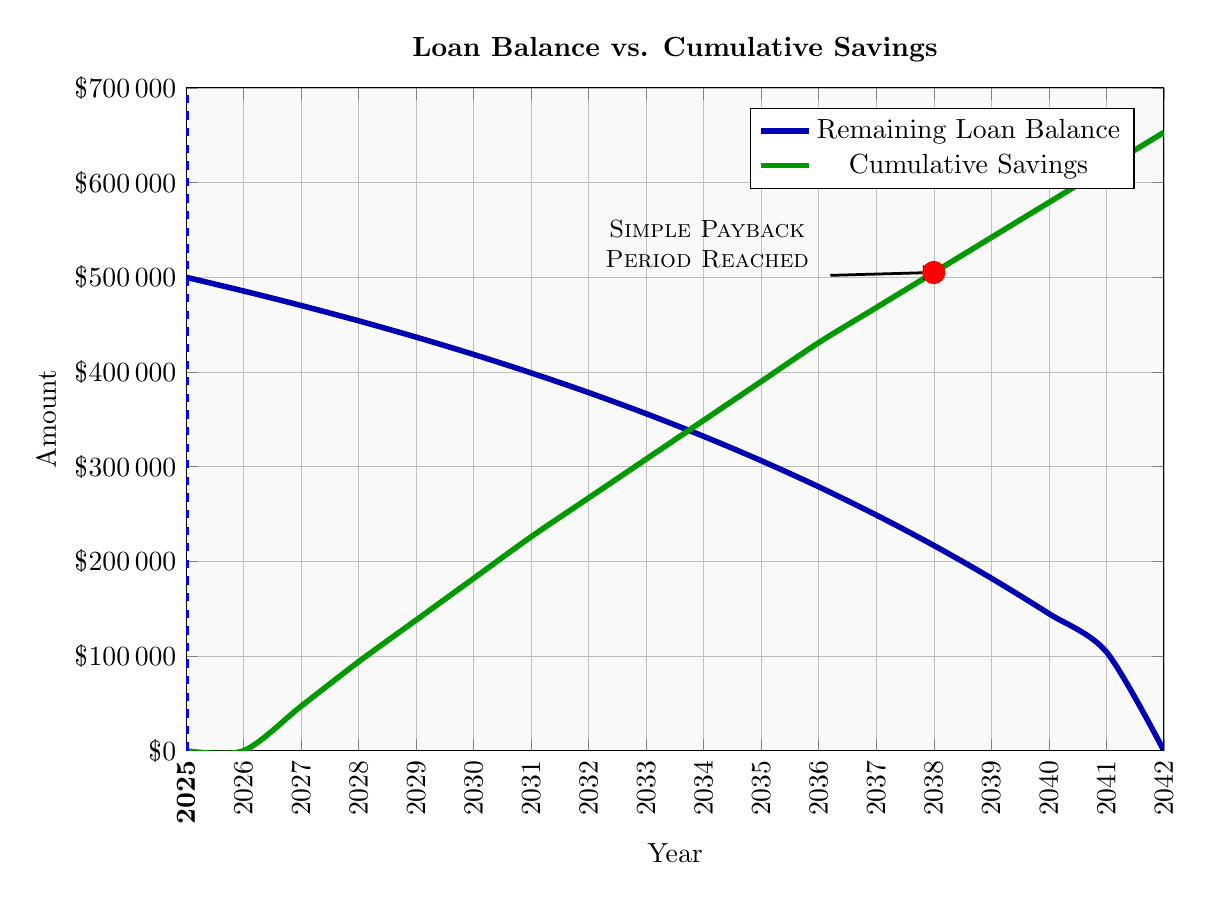
\begin{tikzpicture}
\begin{axis}[
    title={\textbf{Loan Balance vs. Cumulative Savings}},
    xlabel={Year},
    ylabel={Amount},
    xmin=2025, xmax=2042,
    ymin=0, ymax=700000,
    legend pos=north east,
    grid=major,
    grid style={line width=0.1pt, draw=gray!30},
    major grid style={line width=0.2pt, draw=gray!50},
    width=14cm,
    height=10cm,
    axis background/.style={fill=gray!5},
    scaled y ticks=false,
    y tick label style={/pgf/number format/fixed,/pgf/number format/1000 sep=\,},
    yticklabel={\$\pgfmathprintnumber{\tick}},
    xtick={2025,2026,2027,2028,2029,2030,2031,2032,2033,2034,2035,2036,2037,2038,2039,2040,2041,2042},
    x tick label style={rotate=90, anchor=east, /pgf/number format/fixed,/pgf/number format/1000 sep=},
    xticklabels={\textbf{2025},2026,2027,2028,2029,2030,2031,2032,2033,2034,2035,2036,2037,2038,2039,2040,2041,2042}
]

% Realistic loan balance with proper amortization curve
\addplot[color=blue!70!black, line width=2pt, smooth] coordinates {
    (2025, 500000) (2026, 485500) (2027, 470200) (2028, 454000) (2029, 436800)
    (2030, 418500) (2031, 399000) (2032, 378200) (2033, 355900) (2034, 332000)
    (2035, 306300) (2036, 278700) (2037, 248900) (2038, 216800) (2039, 182200) (2040, 144800) (2041, 104400) (2042, 0)
};

% Cumulative savings - no savings in 2025 (upgrade year), savings begin in 2026
\addplot[color=green!60!black, line width=2pt, smooth] coordinates {
    (2025, 0) (2026, 0) (2027, 47000) (2028, 94000) (2029, 138000) (2030, 182000)
    (2031, 226000) (2032, 267000) (2033, 308000) (2034, 349000) (2035, 390000)
    (2036, 431000) (2037, 468000) (2038, 505000) (2039, 542000) (2040, 579000) (2041, 616000) (2042, 653000)
};

% Add marker at payback point
\addplot[only marks, mark=*, mark size=4pt, color=red] coordinates {(2038, 505000)};

% Add professional annotation with arrow
\node[anchor=south east, align=center, font=\small\sffamily] at (axis cs:2036,500000) {
    \textcolor{black}{\textsc{Simple Payback}}\\
    \textcolor{black}{\textsc{Period Reached}}
};
\draw[->, color=black, line width=1pt] (axis cs:2036.2,502000) -- (axis cs:2037.95,505000);

% Upgrade completion vertical line and label
\draw[color=blue, line width=2pt, dashed] (axis cs:2025,0) -- (axis cs:2025,700000);
\node[anchor=south, font=\scriptsize\sffamily, rotate=90, color=blue] at (axis cs:2025,650000) {Upgrade Completed};

\legend{Remaining Loan Balance, Cumulative Savings}

\end{axis}
\end{tikzpicture}
\end{center}

The simple payback period occurs when the green cumulative savings line reaches the loan principal amount of \$500,000. This visualization shows how cumulative savings continue to grow beyond payback, demonstrating the long-term financial benefits of the retrofit investment.

\section{NOI Analysis}

Net Operating Income (NOI) represents the annual income generated by a property after deducting all operating expenses but before deducting taxes and debt service. The methodology uses a unified approach based on rent stabilization status and building characteristics from PLUTO data.

\subsection{NOI Calculation Methodology}

The system uses a three-step process to calculate annual building NOI:

\subsubsection{Step 1: NOI Calculation}

The system uses a three-tier approach based on building class:

\textbf{Cooperative Buildings (Building Classes C0-C9)}

NOI values are obtained directly from the NYC Open Data Cooperative Comparable Rental Income dataset\footnote{NYC Open Data API: https://data.cityofnewyork.us/resource/myei-c3fa.json using \code{net\_operating\_income} field. Data updated periodically by NYC Department of Finance.}:

\begin{equation}
\code{currentNOI} = \text{API}(\text{BBL})[\text{net\_operating\_income}]
\end{equation}

\textbf{Condominium Buildings (Building Classes R4, R5, R6A-R9B, D4-D9)}

NOI values are obtained directly from the NYC Open Data Condominium Comparable Rental Income dataset\footnote{NYC Open Data API: https://data.cityofnewyork.us/resource/9ck6-2jew.json using \code{net\_operating\_income} field. Data updated periodically by NYC Department of Finance.}:

\begin{equation}
\code{currentNOI} = \text{API}(\text{BBL})[\text{net\_operating\_income}]
\end{equation}

\textbf{All Other Residential Buildings (Fallback)}

For buildings not covered by NYC Open Data APIs or where data is not available, NOI is calculated using the 2025 RGB Study data\footnote{Source: \textit{2025 Income and Expense Study}, NYC Rent Guidelines Board, March 2025. Data structured by tenure (stabilized/market rate), location, building age, and size buckets.}. To use this data, we need to determine rent stabilization status and location:

\subsubsection{Step 2: Rent Stabilization Determination}

Determine if the building contains rent stabilized units:

\begin{lstlisting}
function isRentStabilized(bbl: string, pluto: PlutoRecord): boolean {
  // Primary Method: BBL lookup in rent stabilized buildings registry
  if (rentStabilizedBBLs.includes(bbl)) {
    return true;
  }
  
  // Fallback Heuristic: PLUTO-based criteria
  const isPrewar = pluto.yearBuilt > 0 && pluto.yearBuilt < 1974;
  const isHighRise = pluto.numFloors > 6;
  const isNotCondo = pluto.condoNo == null;
  const isNotCoop = !pluto.bldgClass.includes("C6") && !pluto.bldgClass.includes("D4");
  
  return isPrewar && isHighRise && isNotCondo && isNotCoop;
}
\end{lstlisting}

\subsubsection{Step 3: Location Assignment}

Determine the building's location category based on borough and community district (Core Manhattan: CD 101-108; Upper Manhattan: CD 109-112).

\subsubsection{Step 4: Final NOI Calculation}

The NOI per unit per month is obtained from the 2025 RGB Study data using location, rent stabilization status, building era (for stabilized buildings), and size buckets (11-19 units, 20-99 units, 100+ units). Era is determined by: \code{yearBuilt} $\leq$ 1973 $\rightarrow$ \code{pre\_1974}, otherwise \code{post\_1973}. Market rate data is not segmented by building era.

For all buildings, the final annual building NOI is calculated as:

\begin{equation}
\code{annualBuildingNOI} = \code{noiPerUnitPerMonth} \times \code{unitsRes} \times 12
\end{equation}

Where:
\begin{itemize}
    \item \code{noiPerUnitPerMonth}: NOI per residential unit per month from lookup
    \item \code{unitsRes}: Total residential units in building
    \item 12: Months per year conversion factor
\end{itemize}

\subsection{Upgrade Impact on NOI}

The true impact of PTHP upgrades becomes clear when comparing NOI scenarios:

\textbf{Scenario A: No Upgrade (Status Quo)}
\begin{align}
\code{noiNoUpgrade2024to2029} &= \code{currentNOI} - \code{annualFeeExceedingBudget2024to2029}
\end{align}
\begin{align}
\code{noiNoUpgrade2030to2034} &= \code{currentNOI} - \code{annualFeeExceedingBudget2030to2034}
\end{align}
\begin{align}
\code{noiNoUpgradePost2035} &= \code{currentNOI} - \code{annualFeeExceedingBudget2035toFuture}
\end{align}

\textbf{Scenario B: With PTHP Upgrade}
\begin{align}
\code{noiWithUpgrade2024to2027} &= \code{currentNOI} + \code{annualSavingsEnergy} \nonumber\\
&\quad - \code{adjustedAnnualFee2024to2027}
\end{align}
\begin{align}
\code{noiWithUpgrade2027to2029} &= \code{currentNOI} + \code{annualSavingsEnergy} \nonumber\\
&\quad - \code{adjustedAnnualFee2027to2029}
\end{align}
\begin{align}
\code{noiWithUpgrade2030to2034} &= \code{currentNOI} + \code{annualSavingsEnergy} \nonumber\\
&\quad - \code{adjustedAnnualFee2030to2034}
\end{align}
\begin{align}
\code{noiWithUpgradePost2035} &= \code{currentNOI} + \code{annualSavingsEnergy} \nonumber\\
&\quad - \code{adjustedAnnualFee2035toFuture}
\end{align}

\subsection{NOI Calculation Functions}

The NOI calculations can be implemented with unified functions that handle all compliance periods:

\begin{lstlisting}
function calculateAdjustedNOINoUpgrade(year: number): number {
  const currentNOI = await getNoiByBbl(bbl, unitBreakdown); // from NOI API endpoint
  
  if (year >= 2024 && year <= 2029) {
    return currentNOI - annualFeeExceedingBudget2024to2029;
  } else if (year >= 2030 && year <= 2035) {
    return currentNOI - annualFeeExceedingBudget2030to2034;
  } else {
    return currentNOI - annualFeeExceedingBudget2035toFuture;
  }
}

function calculateAdjustedNOIUpgrade(year: number): number {
  const currentNOI = await getNoiByBbl(bbl, unitBreakdown); // from NOI API endpoint
  const energySavings = getEnergySavings();
  
  let reducedLL97Penalties = 0;
  if (year >= 2024 && year <= 2029) {
    reducedLL97Penalties = adjustedAnnualFee2024to2029; // actual penalties paid after upgrade
  } else if (year >= 2030 && year <= 2035) {
    reducedLL97Penalties = adjustedAnnualFee2030to2034; // actual penalties paid after upgrade  
  } else {
    reducedLL97Penalties = adjustedAnnualFee2035toFuture; // actual penalties paid after upgrade
  }
  
  return currentNOI + energySavings - reducedLL97Penalties;
}
\end{lstlisting}

\subsubsection{Implementation Example}

For a 100,000 sq ft rental building with current NOI of \$1,200,000:

\textbf{Without Upgrade:} Building faces ongoing LL97 penalties starting in 2026
\begin{itemize}
    \item 2024-2025: NOI = \$1,200,000 (current NOI) - \$0 (no penalties yet) = \$1,200,000
    \item 2026-2029: NOI = \$1,200,000 (current NOI) - \$150,000 (LL97 penalties paid) = \$1,050,000
    \item 2030-2034: NOI = \$1,200,000 (current NOI) - \$300,000 (LL97 penalties paid) = \$900,000
    \item 2035+: NOI = \$1,200,000 (current NOI) - \$300,000 (LL97 penalties paid) = \$900,000
\end{itemize}

\textbf{With PTHP Upgrade:} Upgrade completes in 2025, savings + reduced penalties start in 2026
\begin{itemize}
    \item 2024-2025: NOI = \$1,200,000 (current NOI) - \$0 (no changes yet) = \$1,200,000
    \item 2026-2027: NOI = \$1,200,000 (current NOI) + \$39,000 (energy savings) - \$15,000 (reduced LL97 penalties) = \$1,224,000
    \item 2030-2034: NOI = \$1,200,000 (current NOI) + \$39,000 (energy savings) - \$33,000 (reduced LL97 penalties) = \$1,206,000  
    \item 2035+: NOI = \$1,200,000 (current NOI) + \$39,000 (energy savings) - \$33,000 (reduced LL97 penalties) = \$1,206,000
\end{itemize}

\subsection{NOI Visualization Over Time}

The following chart shows how NOI evolves differently in upgrade vs no-upgrade scenarios across LL97 compliance periods:

\begin{center}
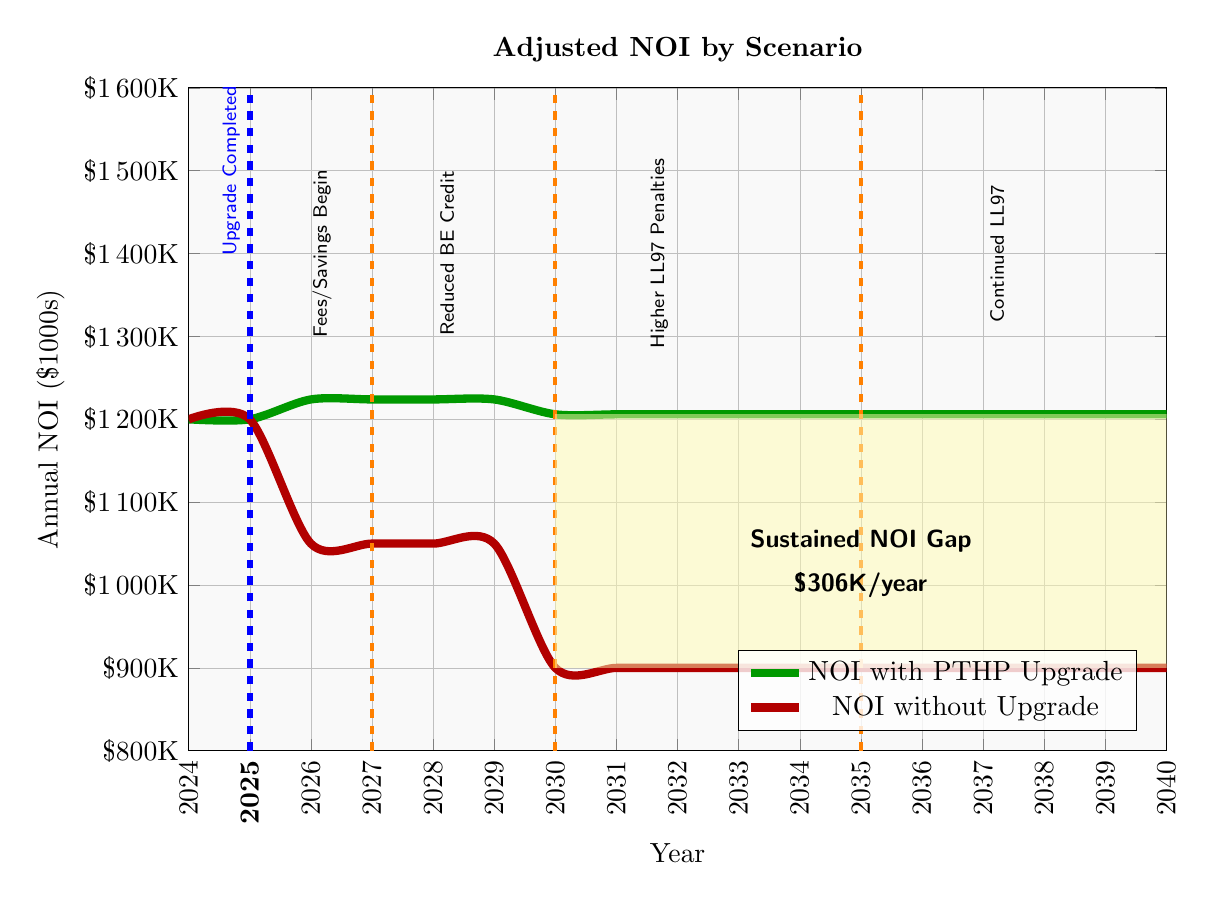
\begin{tikzpicture}
\begin{axis}[
    title={\textbf{Adjusted NOI by Scenario}},
    xlabel={Year},
    ylabel={Annual NOI (\$1000s)},
    xmin=2024, xmax=2040,
    ymin=800, ymax=1600,
    legend pos=south east,
    legend style={draw=black, fill=white, fill opacity=0.8, text opacity=1},
    grid=major,
    grid style={line width=0.1pt, draw=gray!30},
    major grid style={line width=0.2pt, draw=gray!50},
    width=14cm,
    height=10cm,
    axis background/.style={fill=gray!5},
    scaled y ticks=false,
    y tick label style={/pgf/number format/fixed,/pgf/number format/1000 sep=\,},
    yticklabel={\$\pgfmathprintnumber{\tick}K},
    xtick={2024,2025,2026,2027,2028,2029,2030,2031,2032,2033,2034,2035,2036,2037,2038,2039,2040},
    x tick label style={rotate=90, anchor=east, /pgf/number format/fixed,/pgf/number format/1000 sep=},
    xticklabels={2024,\textbf{2025},2026,2027,2028,2029,2030,2031,2032,2033,2034,2035,2036,2037,2038,2039,2040}
]

% NOI with PTHP upgrade - upgrade completes in 2025, savings start in 2026
\addplot[color=green!60!black, line width=3pt, smooth] coordinates {
    (2024, 1200) (2025, 1200) (2026, 1224) (2027, 1224) (2028, 1224) (2029, 1224)
    (2030, 1206) (2031, 1206) (2032, 1206) (2033, 1206) (2034, 1206)
    (2035, 1206) (2036, 1206) (2037, 1206) (2038, 1206) (2039, 1206) (2040, 1206)
};

% NOI without upgrade - dramatic drop in 2026 when LL97 fees kick in
\addplot[color=red!70!black, line width=3pt, smooth] coordinates {
    (2024, 1200) (2025, 1200) (2026, 1050) (2027, 1050) (2028, 1050) (2029, 1050)
    (2030, 900) (2031, 900) (2032, 900) (2033, 900) (2034, 900)
    (2035, 900) (2036, 900) (2037, 900) (2038, 900) (2039, 900) (2040, 900)
};

% Add period markers
\draw[color=blue, line width=2pt, dashed] (axis cs:2025,800) -- (axis cs:2025,1600);
\draw[color=orange, line width=1.5pt, dashed] (axis cs:2027,800) -- (axis cs:2027,1600);
\draw[color=orange, line width=1.5pt, dashed] (axis cs:2030,800) -- (axis cs:2030,1600);
\draw[color=orange, line width=1.5pt, dashed] (axis cs:2035,800) -- (axis cs:2035,1600);

% Upgrade completion label
\node[anchor=south, font=\scriptsize\sffamily, rotate=90, color=blue] at (axis cs:2025,1500) {Upgrade Completed};

% Period labels
\node[anchor=south, font=\scriptsize\sffamily, rotate=90] at (axis cs:2026.5,1400) {Fees/Savings Begin};
\node[anchor=south, font=\scriptsize\sffamily, rotate=90] at (axis cs:2028.5,1400) {Reduced BE Credit};
\node[anchor=south, font=\scriptsize\sffamily, rotate=90] at (axis cs:2032,1400) {Higher LL97 Penalties};
\node[anchor=south, font=\scriptsize\sffamily, rotate=90] at (axis cs:2037.5,1400) {Continued LL97};

% Highlight the NOI gap in critical period and beyond
\fill[yellow!30, opacity=0.5] (axis cs:2030,900) rectangle (axis cs:2040,1206);
\node[anchor=center, font=\small\sffamily, color=black] at (axis cs:2035,1053) {\textbf{Sustained NOI Gap}};
\node[anchor=center, font=\small\sffamily, color=black] at (axis cs:2035,1000) {\textbf{\$306K/year}};

\legend{NOI with PTHP Upgrade, NOI without Upgrade}

\end{axis}
\end{tikzpicture}
\end{center}

This NOI comparison reveals the true financial impact of upgrade timing:
\begin{itemize}
    \item \textbf{Immediate NOI Boost}: Upgrading in 2024 increases NOI by \$174K/year (17\% increase)
    \item \textbf{Penalty Avoidance}: Without upgrade, NOI drops \$150K in 2030+ due to higher penalties  
    \item \textbf{Perpetual Benefit}: The \$306K annual NOI gap continues indefinitely post-2035, creating sustained property value advantages
    \item \textbf{Risk Mitigation}: Upgrading protects against declining property values from ongoing LL97 penalties
    \item \textbf{Optimal Window}: Early upgrade (2024-2027) captures maximum BE Credit and avoids penalty escalation
    \item \textbf{Long-term Value}: LL97 compliance continues post-2035, making upgrade benefits permanent rather than temporary
\end{itemize}

\section{Property Value Analysis}

Property values are calculated by dividing NOI by the cap rate, providing a direct correlation between operational performance improvements and asset valuation.

\subsection{Property Value Calculation Functions}

Property value calculations use the same scenarios as NOI but apply cap rate conversion:

\begin{lstlisting}
function calculatePropertyValueNoUpgrade(year: number, capRate: number = 0.04): number {
  const adjustedNOI = calculateAdjustedNOINoUpgrade(year); // NOI minus actual LL97 penalties paid
  return adjustedNOI / capRate;
}

function calculatePropertyValueUpgrade(year: number, capRate: number = 0.04): number {
  const adjustedNOI = calculateAdjustedNOIUpgrade(year); // NOI plus energy savings minus reduced LL97 penalties
  return adjustedNOI / capRate;
}
\end{lstlisting}

The default cap rate of 4\% reflects typical NYC multifamily properties\footnote{Cap rate of 4\% used for NYC multifamily properties. This parameter can be adjusted based on market conditions, property characteristics, and investment criteria.}.

\subsection{Property Value Impact Analysis}

Using a 4\% cap rate typical for NYC multifamily properties:

\textbf{No Upgrade Property Values}
\begin{align}
\code{propertyValueNoUpgrade} &= \code{noiNoUpgrade} \div 0.04
\end{align}

\textbf{With Upgrade Property Values}  
\begin{align}
\code{propertyValueWithUpgrade} &= \code{noiWithUpgrade} \div 0.04
\end{align}

\textbf{Net Property Value Impact}
\begin{align}
\code{netPropertyValueGain} &= \code{propertyValueWithUpgrade} - \code{propertyValueNoUpgrade}
\end{align}

\subsubsection{Implementation Example}

For a 100,000 sq ft rental building with current NOI of \$1,200,000:

\textbf{Without Upgrade:} Building faces ongoing LL97 penalties starting in 2026
\begin{itemize}
    \item 2024-2025: Property Value = \$1,200,000 (NOI) ÷ 0.04 (cap rate) = \$30.0M
    \item 2026-2029: Property Value = \$1,050,000 (NOI) ÷ 0.04 (cap rate) = \$26.25M
    \item 2030-2034: Property Value = \$900,000 (NOI) ÷ 0.04 (cap rate) = \$22.5M
    \item 2035+: Property Value = \$900,000 (NOI) ÷ 0.04 (cap rate) = \$22.5M
\end{itemize}

\textbf{With PTHP Upgrade:} Upgrade completes in 2025, value increases in 2026
\begin{itemize}
    \item 2024-2025: Property Value = \$1,200,000 (NOI) ÷ 0.04 (cap rate) = \$30.0M
    \item 2026-2027: Property Value = \$1,224,000 (NOI) ÷ 0.04 (cap rate) = \$30.6M
    \item 2030-2034: Property Value = \$1,206,000 (NOI) ÷ 0.04 (cap rate) = \$30.15M  
    \item 2035+: Property Value = \$1,206,000 (NOI) ÷ 0.04 (cap rate) = \$30.15M
\end{itemize}

\textbf{Net Property Value Gain:} \$30.15M - \$22.5M = \$7.65M

This \$7.65M property value increase far exceeds typical retrofit costs of \$500K-\$2M, demonstrating the compelling financial case for upgrading.

\subsection{Property Value Impact Visualization}

The following chart demonstrates property value trajectories for both scenarios:

\begin{center}
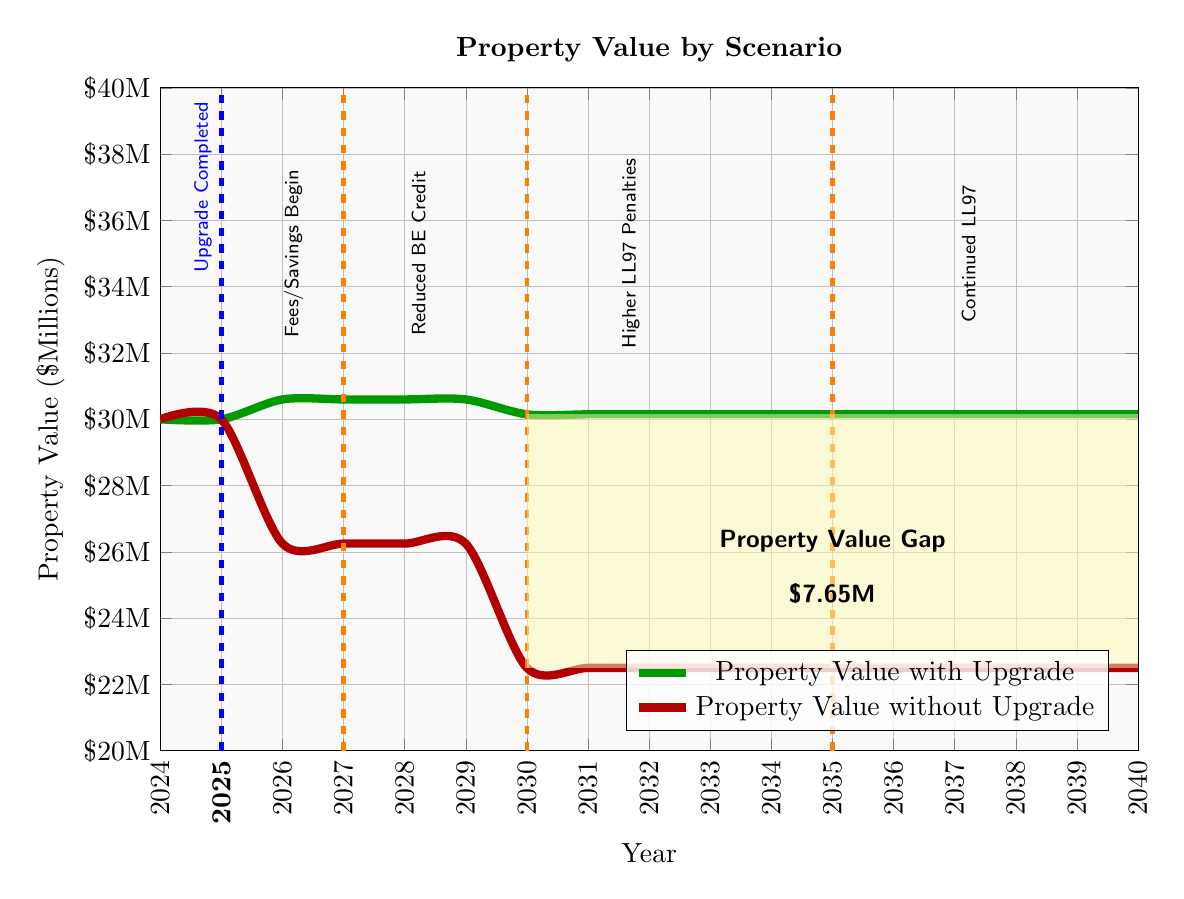
\begin{tikzpicture}
\begin{axis}[
    title={\textbf{Property Value by Scenario}},
    xlabel={Year},
    ylabel={Property Value (\$Millions)},
    xmin=2024, xmax=2040,
    ymin=20, ymax=40,
    legend pos=south east,
    legend style={draw=black, fill=white, fill opacity=0.8, text opacity=1},
    grid=major,
    grid style={line width=0.1pt, draw=gray!30},
    major grid style={line width=0.2pt, draw=gray!50},
    width=14cm,
    height=10cm,
    axis background/.style={fill=gray!5},
    scaled y ticks=false,
    y tick label style={/pgf/number format/fixed,/pgf/number format/1000 sep=\,},
    yticklabel={\$\pgfmathprintnumber{\tick}M},
    xtick={2024,2025,2026,2027,2028,2029,2030,2031,2032,2033,2034,2035,2036,2037,2038,2039,2040},
    x tick label style={rotate=90, anchor=east, /pgf/number format/fixed,/pgf/number format/1000 sep=},
    xticklabels={2024,\textbf{2025},2026,2027,2028,2029,2030,2031,2032,2033,2034,2035,2036,2037,2038,2039,2040}
]

% Property value with PTHP upgrade - upgrade completes in 2025, value increases in 2026
\addplot[color=green!60!black, line width=3pt, smooth] coordinates {
    (2024, 30.0) (2025, 30.0) (2026, 30.6) (2027, 30.6) (2028, 30.6) (2029, 30.6)
    (2030, 30.15) (2031, 30.15) (2032, 30.15) (2033, 30.15) (2034, 30.15)
    (2035, 30.15) (2036, 30.15) (2037, 30.15) (2038, 30.15) (2039, 30.15) (2040, 30.15)
};

% Property value without upgrade - dramatic drop in 2026 when LL97 fees kick in
\addplot[color=red!70!black, line width=3pt, smooth] coordinates {
    (2024, 30.0) (2025, 30.0) (2026, 26.25) (2027, 26.25) (2028, 26.25) (2029, 26.25)
    (2030, 22.5) (2031, 22.5) (2032, 22.5) (2033, 22.5) (2034, 22.5)
    (2035, 22.5) (2036, 22.5) (2037, 22.5) (2038, 22.5) (2039, 22.5) (2040, 22.5)
};

% Period markers
\draw[color=blue, line width=2pt, dashed] (axis cs:2025,20) -- (axis cs:2025,40);
\draw[color=orange, line width=1.5pt, dashed] (axis cs:2027,20) -- (axis cs:2027,40);
\draw[color=orange, line width=1.5pt, dashed] (axis cs:2030,20) -- (axis cs:2030,40);
\draw[color=orange, line width=1.5pt, dashed] (axis cs:2035,20) -- (axis cs:2035,40);

% Upgrade completion label
\node[anchor=south, font=\scriptsize\sffamily, rotate=90, color=blue] at (axis cs:2025,37) {Upgrade Completed};

% Period labels
\node[anchor=south, font=\scriptsize\sffamily, rotate=90] at (axis cs:2026.5,35) {Fees/Savings Begin};
\node[anchor=south, font=\scriptsize\sffamily, rotate=90] at (axis cs:2028.5,35) {Reduced BE Credit};
\node[anchor=south, font=\scriptsize\sffamily, rotate=90] at (axis cs:2032,35) {Higher LL97 Penalties};
\node[anchor=south, font=\scriptsize\sffamily, rotate=90] at (axis cs:2037.5,35) {Continued LL97};

% Highlight the value gap
\fill[yellow!30, opacity=0.5] (axis cs:2030,22.5) rectangle (axis cs:2040,30.15);
\node[anchor=center, font=\small\sffamily, color=black] at (axis cs:2035,26.325) {\textbf{Property Value Gap}};
\node[anchor=center, font=\small\sffamily, color=black] at (axis cs:2035,24.75) {\textbf{\$7.65M}};

\legend{Property Value with Upgrade, Property Value without Upgrade}

\end{axis}
\end{tikzpicture}
\end{center}

This visualization demonstrates the substantial and sustained property value advantage of upgrading, with the \$7.65M gap representing the permanent value creation from PTHP installation.

\section{Implementation Notes}

All variables in the codebase follow camelCase naming convention with the appropriate PTAC or PTHP suffix for clarity. The calculations are implemented in the backend services using TypeScript, ensuring type safety and consistent naming across the platform.

\end{document}